\documentclass[10pt]{article}
\usepackage{amssymb,indentfirst,listings,color,amsmath}
\usepackage{graphicx,epstopdf}
\usepackage[margin=1.5in]{geometry}
\usepackage{caption}
\usepackage{subcaption}
\usepackage{float}
\input{../RJLmacros}

\title{\textbf{Models of Traffic Flow with Discontinuous and Non-convex Flux}}
\author{Qi Guo, Peng Zheng}
\date{}
\begin{document}
\maketitle

\begin{abstract}
In this project, we investigate two models of traffic flow based on Lighthill-Whitham-Richards model. In the first part, we look into the model of traffic flow on freeway, where the flux function is discontinuous and piecewise linear. We utilize the method of mollification to smooth out the discontinuity, and construct the convex hull to solve the problem. Additionally, a numerical PDE solver in CLAWPACK and a ODE solver of car-following model are designed to simulate the results. In the second part, the car-following model of night-time driving is explored. With or without perturbing the velocities, we could observe the instability and clustering of cars with uniform initial density.
\end{abstract}
%-----------------------------------------------------------------------------------------------------------------------%
\section{Introduction}

In 1950's, Lighthill, Whitham and Richards proposed a model, now known as LWR model, for traffic flow problem. Specifically, this model is a scalar hyperbolic nonlinear equation satisfying conservation law:

\[
\rho_t+f(\rho)_x=0,
\]
where $f(\rho)=\rho v(\rho)$ and the normalized vehicle density $\rho$ is within the range of $[0,1]$.

\vskip 8pt

In \cite{WS}, Wiens, Stockie and Williams discussed a flux function with discontinuity at a single point $\rho_m$. This flux function is fitted by empirical dataset collected from freeway. In the first part of project, our goals are to smooth out the flux function, construct the exact solution, solve the problem numerically, and compare solutions with the car-following model.

\vskip 8pt

In the second part of this paper, the night-time driving model in \cite{RJ} is discussed. The night-time model has interesting features, one of which is the clustering behavior of cars.
As in the first part, we implement an ODE solver for car-following model. Additionally, we compare with a couple of initial densities,
 and perturb velocities randomly to observe the different clustering behavior.
%-----------------------------------------------------------------------------------------------------------------------%
\section{Freeway Model}
%----------------------------------------------------------
\subsection{Overview}

The freeway model consists the scalar conservation law:
\[
\rho_t + f(\rho)_x = 0
\]
with flux function
 \[f(\rho)=\left\{
  \begin{array}{l l}
   \rho \ \ \ &\text{if}\ \  0\leq \rho <\rho_m,\\
    \gamma(1-\rho) \ \ \ &\text{if}\ \ \rho_m\leq\rho\leq 1.
  \end{array} \right.\]

  From the empirical data, we set $\rho_m>\gamma(1-\rho_m)$, which indicates
  \[
  0<\gamma<\frac{\rho_m}{1-\rho_m}.
  \]

\hfil\includegraphics[width=4in]{./figs/freeway_flux_original.eps}

  The flux function is discontinuous at $\rho_m$. If we want to solve this equation explicitly as in continuous case, then the discontinuity has to be dealt with,
  which leads to the method of mollification.
%----------------------------------------------------------
\subsection{Method of Mollification}

We will utilize the method of mollification in this section. Particularly, we want to have this form to solve:
\[
\frac{\partial \rho}{\partial t} + \frac{\partial f_\epsilon(\rho)}{\partial x} = 0,
\]
where $f_\epsilon(\rho)$ is a continuous function in $[0,1]$. By using mollification, this function is called mollified flux function.
\vskip 8pt
The mollified flux function can be constructed as the convolution of original flux function and mollifier:
\[
f_\epsilon=\eta_\epsilon\ast f.
\]
Explicitly,
\begin{equation}\nonumber
f_{\epsilon}(\rho_{\epsilon})=\rho_{\epsilon}+(\gamma-(\gamma+1)\rho_{\epsilon})\int_{\rho_m-\epsilon}^{\rho_{\epsilon}} \eta_\epsilon(s-\rho_\epsilon) ds
\label{eq:flux}
\end{equation}

\hfil\includegraphics[width=4in]{./figs/freeway_flux_mollified.eps}

with $0<\epsilon\ll 1$. The mollifier function is $\eta_\epsilon(s)=\frac{1}{\epsilon}\eta(s/\epsilon)$, where $\eta(s)$ is called mollifier, satisfying:
\\\\
(1) $\eta\geq 0$;\\
(2) $\eta$ has smooth derivatives of any order, and also compactly supported on $[-1,1]$;\\
(3) $\eta(-s)=\eta(s)$ for all real $s$;\\
(4) $\int_{-\infty}^{\infty} \eta(s) ds=1$.
\\\\

A canonical mollifier $\eta$ is:
 \[\eta(s)=\left\{
  \begin{array}{l l}
    C\exp(1/(s^2-1)) \ \ \ &\text{if}\ \ |s|<1\\
    0 \ \ \ &\text{if}\ \ |s|\geq 1
  \end{array} \right.\]

  With the 4th condition of this function, we can obtain $C\approx2.2522836.$ Now it is reasonable to use the standard tools to solve the mollified problem.
  In \cite{DF}, it has been proved that solutions to mollified problem converge to solutions to the original problem as $\epsilon\rightarrow 0$.
%----------------------------------------------------------
%\subsection{Anisotropic Flows and Entropy Condition}

%Drivers mainly focus on the vehicles in front of them. This phenomenon is called anisotropic, which is very different from gas dynamics or acoustics. Hence %models based on fluid dynamics, where Oleinik's entropy condition dominates, which is
%\[
%\text{TO BE ADDED}
%\]
% often violate the anisotropic behavior in traffic flow, see [EEE].
%\vskip 8pt
%Zhang set two mathematical criteria for anisotropic in [FFF], and Wiens proved that this model also satisfies the anisotropic criteria in [GGG]. Even though %there are reasons to resist Oleinik's condition, this criterion still provides reasonable solution to this problem.

%----------------------------------------------------------
\subsection{Exact Solution, Numerical Solution and Car-following Model}
\subsubsection{Convexity of Mollified Flux}

The flux function is Equation (\ref{eq:flux}). We can calculate its first and second derivative:
\[
f'_\epsilon(\rho_\epsilon)=1+[\gamma-(\gamma+1)
\rho_\epsilon]\eta_\epsilon(\rho_\epsilon-\rho_m)-(\gamma+1)\int_{\rho_m-\epsilon}^{\rho_\epsilon}\eta_\epsilon(s-\rho_m) ds
\]
and
\[
f''_\epsilon(\rho_\epsilon)=G(\rho_\epsilon)P(\rho_\epsilon),
\]
where
\[G(\rho_\epsilon)=\frac{2\eta_\epsilon(\rho_\epsilon-\rho_m)}{\epsilon^2(\gamma+1)[(\frac{\rho_\epsilon-\rho_m}{\epsilon})^2-1]^2},
\]
and
\[P(\rho_\epsilon)=(\frac{\gamma}{\gamma+1}-\rho_\epsilon)(\rho_m-\rho_\epsilon)-\epsilon^2[(\frac{\rho_\epsilon-\rho_m}{\epsilon})^2-1]^2.
\]

Since $G(\rho_\epsilon)\geq 0$, thus we only need to focus on $P(\rho_\epsilon)$. It has been proven in \cite{WS} that $f''(\rho_\epsilon)\geq 0$ when $\rho_\epsilon\in [\rho_m,1]$, and $f''_\epsilon(\rho_\epsilon)\leq 0$ when $\rho_\epsilon\in[0,\rho_m]$.

\subsubsection{Convex-Hull Method}

To determine the weak solution to a non-convex scalar conservation law, in this particular problem, we will use Olenik's entropy condition:

\[
\frac{f(\rho)-f(\rho_l)}{\rho-\rho_l}\geq \frac{f(\rho_l)-f(\rho_r)}{\rho_l-\rho_r}\geq \frac{f(\rho)-f(\rho_r)}{\rho-\rho_r}
\]

for all $\rho$ between $\rho_l$ and $\rho_r$.
\vskip 8pt
The entropy-satisfying solution can be determined form the graph of $f_\epsilon(\rho)$. This method is called convex hull.
\vskip 8pt

In the following part of this section, we will use convex-hull method to solve this problem, with three sets of initial conditions.
\subsubsection{Numerical Solution}
To implement the numerical solution of the mollified problem, we use the second order Lax-Wendroff method with Van Leer limiter in CLAWPACK.

\vskip 8pt
We set up $\gamma=0.5$, $\rho_m=0.5$, $\epsilon=0.01$ in numerical solution.
\subsubsection{Car-Following Model}
If we take
\[\rho_k=\frac{1}{X_{k+1}-X_{k}},\]
and for $k$th car, then there are $m$ nonlinear equations:
\[
X_k'(t)=v_n(t)=U(\rho_k(t)).
\]
Also, the position of each car is updated by
\[
x_{n}(t+\Delta t)=x_{n}(t)+v_{n}(t)\Delta t.
\]
for $k=1,2,...,m$, where $m$ is the number of cars and $U$ is the velocity function.


\subsubsection{Exact Solutions and Experiments}
%---------------------------------------------
{\bf Case 1} ($\rho_r<\rho_m<\rho_l$)
\\

We can construct the smallest convex-hull of $\{(\rho_\epsilon,y):\ \rho_r<\rho_\epsilon<\rho_l \ \text{and}\ y\leq f_\epsilon(\rho_\epsilon)\}$. The shock speed is:
\[
s = \frac{f_\epsilon(\rho_l)-f_\epsilon(\rho_\ast)}{\rho_l-\rho_\ast}=f'_\epsilon(\rho_\ast),
\]
where $\rho_\ast\in(\rho_m-\epsilon,\rho_m)$.
\vskip 8pt
When $\epsilon\rightarrow 0$, the rarefaction wave flattens out and reduces to the constant state $\rho_m$. The limiting solution is:

$$\rho(x,t)=\left\{
  \begin{array}{l l}
   \rho_l \ \ \ &\text{if}\ \  x < st,\\
   \rho_m \ \ \ &\text{if}\ \ st \leq x \leq  t,\\
   \rho_r \ \ \ &\text{if}\ \ x > t.
\end{array} \right.$$

Here we set $\rho_l=0.9$, $\rho_r=0.2$.
\vskip 1cm

\begin{itemize}
   \item  Numerical Results:
 \end{itemize}

\hfil\includegraphics[width=2.5in]{./figs/initial_condition_1/frame0000fig1.eps}
\includegraphics[width=2.5in]{./figs/initial_condition_1/frame0001fig1.eps} \hfil

\begin{itemize}
   \item  Car-following Model:
 \end{itemize}
 %\hspace*{-1.0in}
 \hfil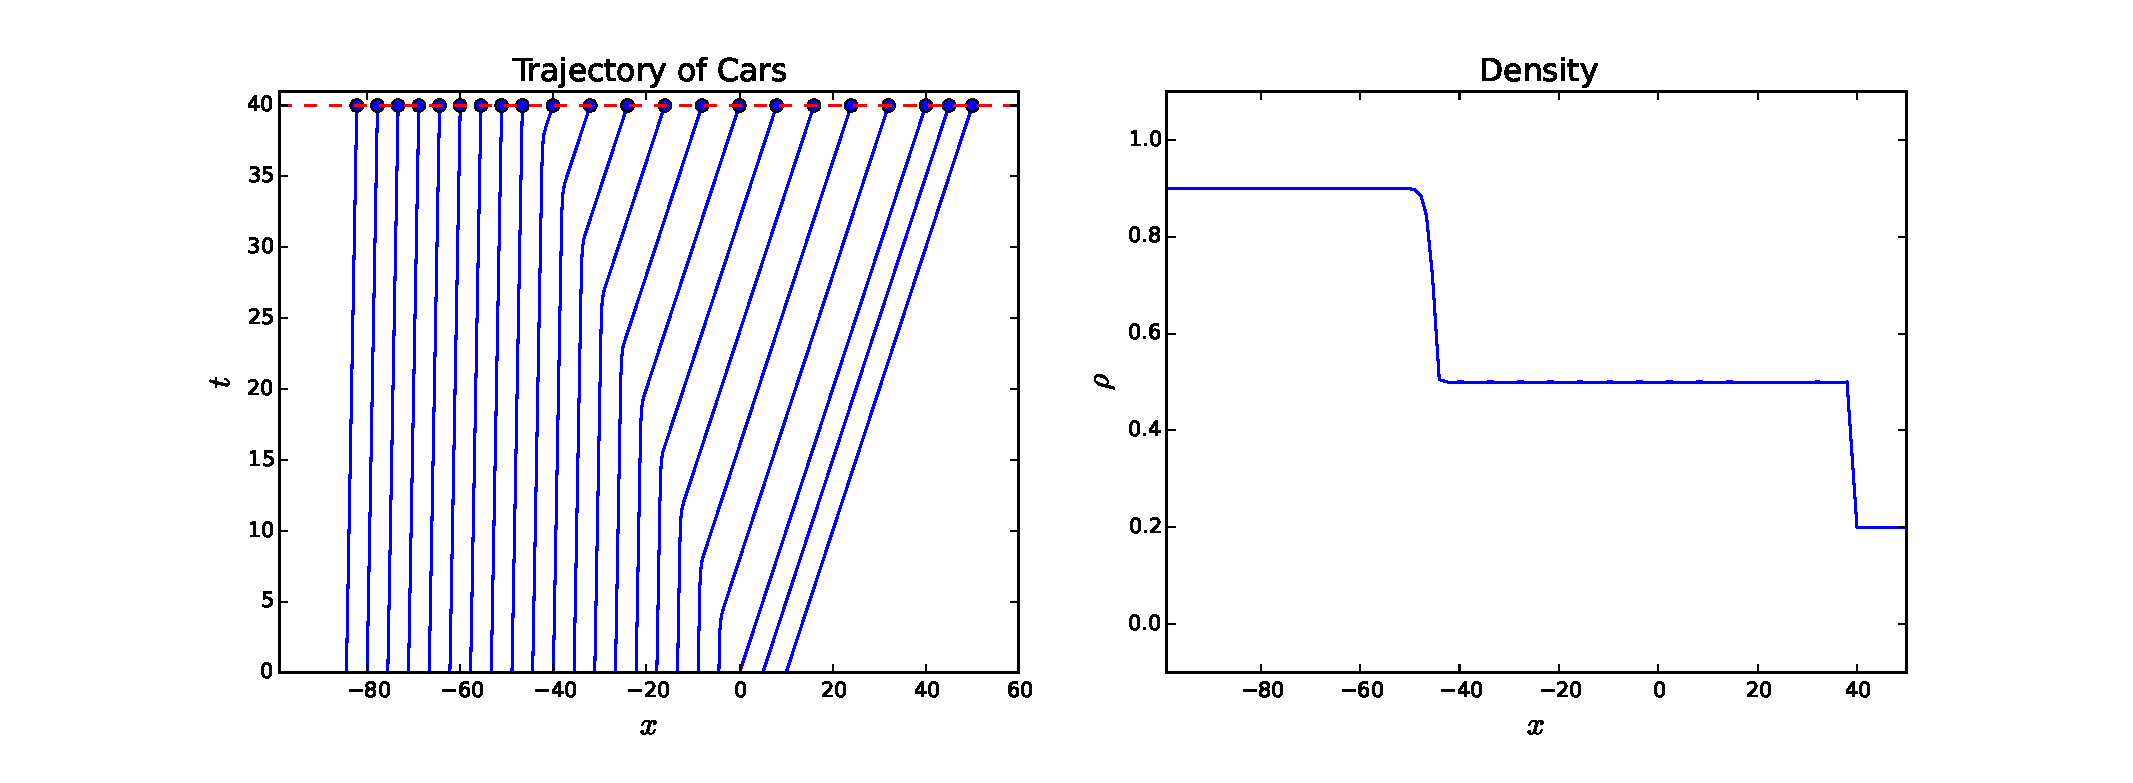
\includegraphics[width=5.7in]{./figs/initial_condition_1/_plots_ode_freeway1_80.eps}\hfil
%---------------------------------------------
{\bf Case 2} ($\frac{\gamma}{\gamma+1}<\rho_l<\rho_m<\rho_r$)
\\

Here, we construct the smallest convex hull of the set $\{(\rho,y):\rho_l<\rho<\rho_r,\ \text{and}\ y\geq f_\epsilon(\rho)\}$.
It is clear that, $\rho=\frac{\gamma}{\gamma+1}$ is a critical point where the convex-hull behaves differently, by calculating the intersection of two pieces of original flux function.
\vskip 8pt

When $\epsilon\rightarrow 0$, the rarefaction wave flattens out and reduces to the constant state $\rho_m$. The limiting solution is:

$$\rho(x,t)=\left\{
  \begin{array}{l l}
   \rho_l \ \ \ &\text{if}\ \  x < st,\\
   \rho_m \ \ \ &\text{if}\ \ st \leq x \leq -\gamma t,\\
   \rho_r \ \ \ &\text{if}\ \ x > -\gamma t,
\end{array} \right.$$

  where $s=\frac{f_\epsilon(\rho_\ast)-f_\epsilon(\rho_l)}{\rho_\ast-\rho_l}=f'_\epsilon(\rho_{\ast})$, and $\rho\in(\rho_m-\epsilon,\rho_m)$.
\vskip 8pt
  Here we set $\rho_l=0.4$, $\rho_r=0.9$.

\vskip 1cm

\begin{itemize}
   \item  Numerical Results:
 \end{itemize}

\hfil\includegraphics[width=2.5in]{./figs/initial_condition_2/frame0000fig1.eps}
\includegraphics[width=2.5in]{./figs/initial_condition_2/frame0001fig1.eps} \hfil

\begin{itemize}
   \item  Car-following Model:
 \end{itemize}
 %\hspace*{-1.0in}
 \hfil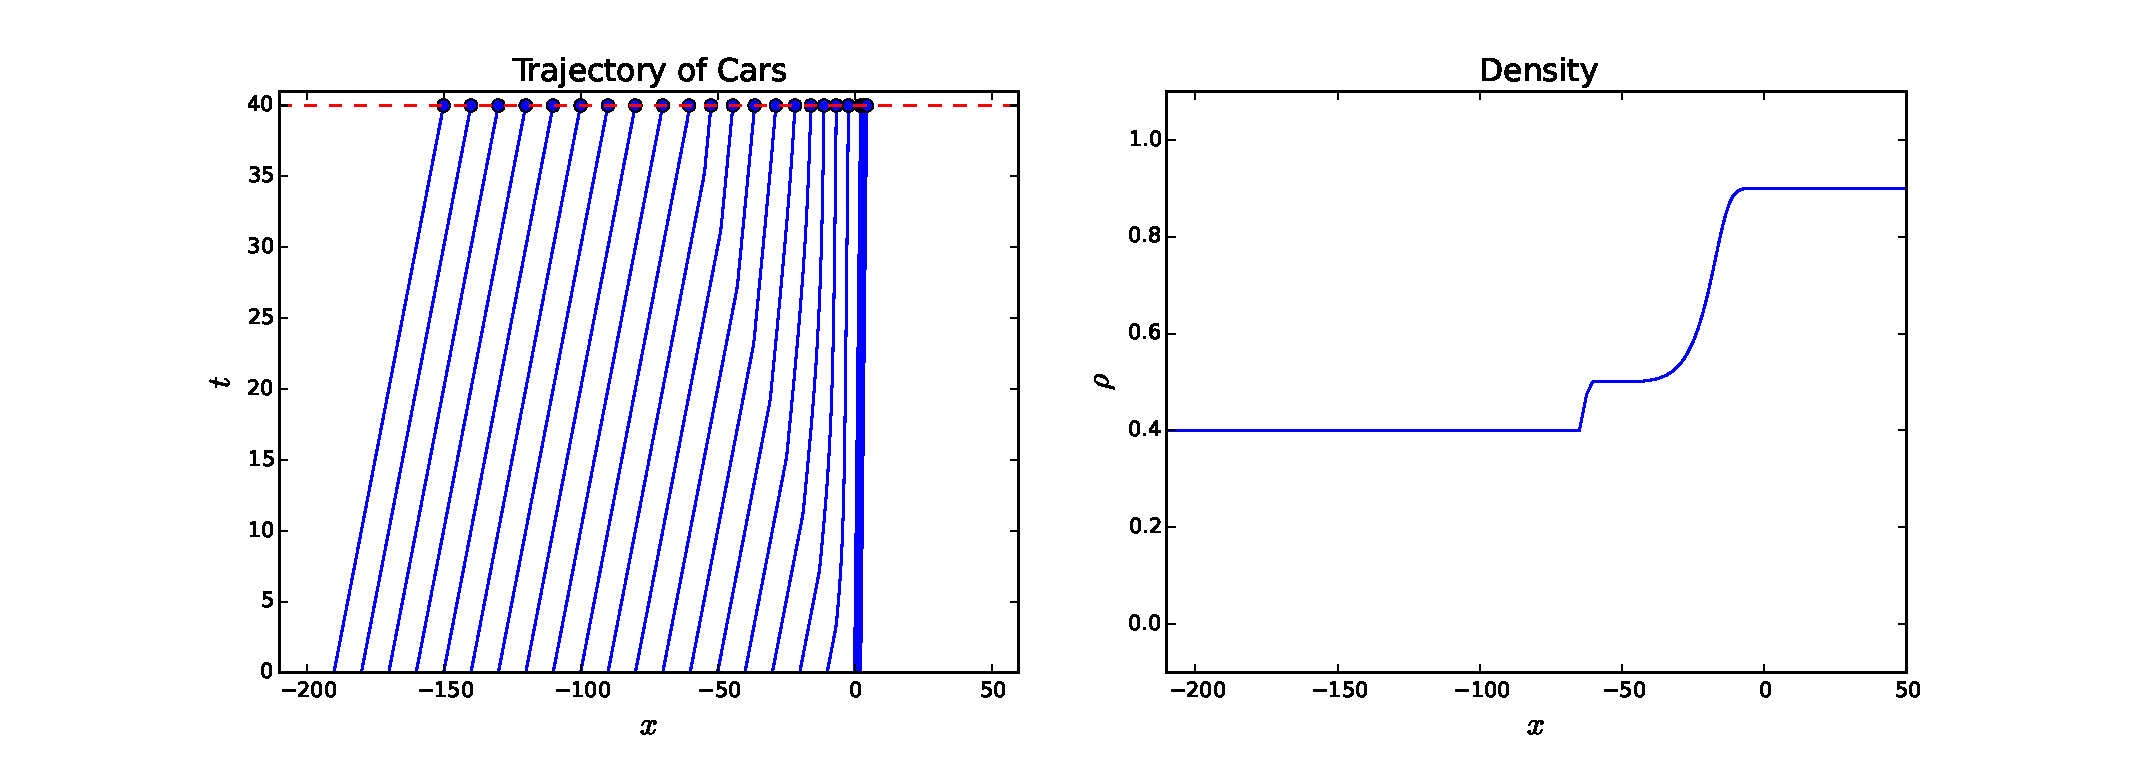
\includegraphics[width=5.7in]{./figs/initial_condition_2/_plots_ode_freeway2_80.eps}\hfil
%---------------------------------------------
{\bf Case 3} ($\rho_l<\rho_m<\rho_r$ and $\frac{\gamma}{\gamma+1}\geq \rho_l$)
\\

We construct the same convex hull as case 2. Since $\frac{\gamma}{\gamma+1}\geq \rho_l$, there is only a shock in this solution.

$$\rho(x,t)=\left\{
  \begin{array}{l l}
   \rho_l \ \ \ &\text{if}\ \  x < st,\\
   \rho_r \ \ \ &\text{if}\ \ x > st,
\end{array} \right.$$

  where $s=\frac{f_\epsilon(\rho_r)-f_\epsilon(\rho_l)}{\rho_r-\rho_l}.$
\vskip 8pt
  Here we set $\rho_l=0.2$, $\rho_r=0.9$.
\vskip 1cm
  
  \begin{itemize}
   \item  Numerical Results:
 \end{itemize}

\hfil\includegraphics[width=2.5in]{./figs/initial_condition_3/frame0000fig1.eps}
\includegraphics[width=2.5in]{./figs/initial_condition_3/frame0001fig1.eps} \hfil

\begin{itemize}
   \item  Car-following Model:
 \end{itemize}
 %\hspace*{-1.0in}
 \hfil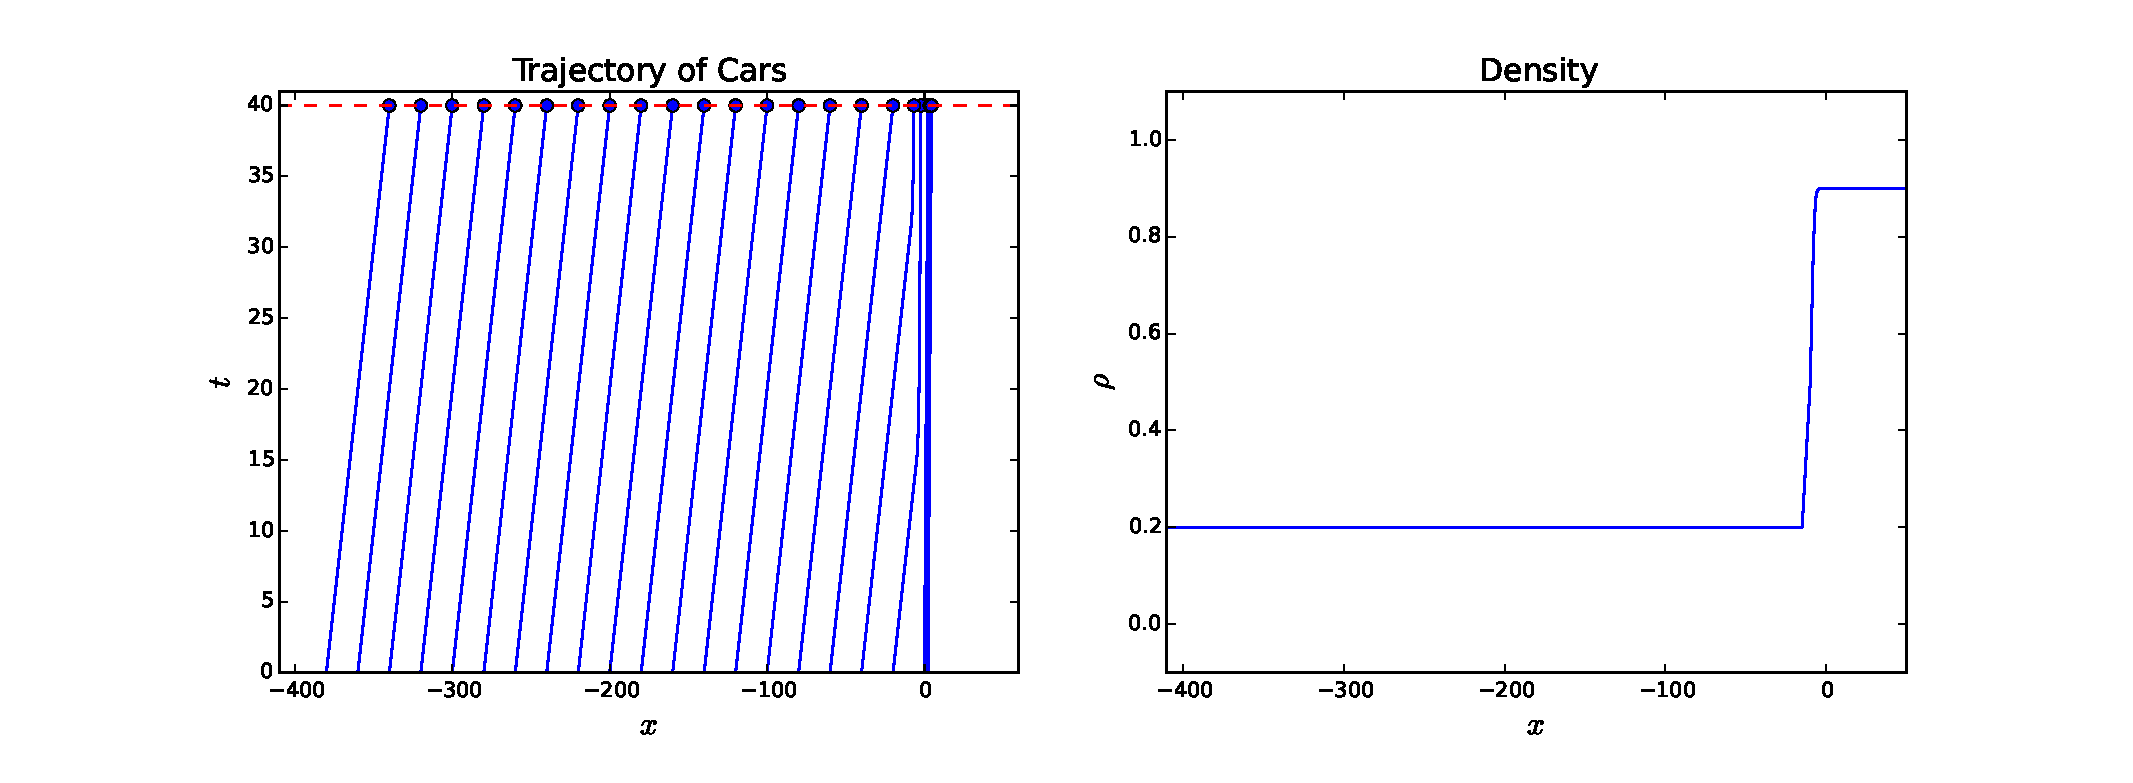
\includegraphics[width=5.7in]{./figs/initial_condition_3/_plots_ode_freeway3_80.eps}\hfil
%----------------------------------------------------------
\subsection{Discussion}

In the previous section, we compared with three different methods for this problem.
\vskip 8pt
It is clear that the variation of density in car-following model complies with both the exact solution and the
numerical solution of mollified problem in all the three cases.
\vskip 8pt
For numerical experiment, in the first case, since two discontinuities are moving to opposite directions, it is natural to consider the entropy fix condition of transonic rarefaction when designing
 the PDE solver. For other two cases, we can design PDE solver as normal. The errors of numerical solutions are acceptable.
%-----------------------------------------------------------------------------------------------------------------------%
\section{Night-time Driving Model}
%----------------------------------------------------------
\subsection{Overview}

We have a different flux function in the night-time driving model.
\vskip 8pt
When cars are driving at night on mountain road, the speed limitation is needed for safe driving if there are no cars ahead. For example, drivers may not know the road conditions.
Nevertheless, if other cars are driving ahead, fast-driving is safer and easier, since tail lights in front of the driver can be used to indicate how the road twists and turns.
%----------------------------------------------------------
\subsection{Mathematical Model}

LWR model is still used here with flux function,
\[
U(\rho)=\left\{\begin{array}{lll}U_0&\text{if }\rho<\rho_a,\\
c\rho&\text{if }\rho_a\leq\rho\leq\rho_b,\\
U_1(1-\rho)&\text{if }\rho>\rho_b.\end{array}\right.
\]
Here we have $U_{\max}=\frac{\rho_b U_0}{\rho_a}$, $c=\frac{U_{\max}-U_0}{\rho_b-\rho_a}$ and $U_1=\frac{U_{\max}}{1-\rho_b}$.
\vskip 8pt
Velocity stays at some constant value $U_0$ when the density is low,
increases as density increases to $U_{\max}$, but then decreases when the cars are severely congested.

\hspace*{-1.0in}
\hfil\includegraphics[width=7in]{./figs/night_velocity_flux.eps}
%----------------------------------------------------------
\subsection{Clustering Behavior}

When uniformly spaced cars (constant distance $\Delta^0$) face empty road initially, ``clustering'' of cars could be observed. This behavior is due to the non-convexity of the flux. When $\rho_a\leq\rho\leq\rho_b$, uniformly spaced traffic with headway $\Delta^0$ traveling at speed $U(1/\Delta t^0)$ is unstable to small perturbations.
%----------------------------------------------------------
\vskip 1cm

{\bf Car-Following Model}
\\

In the car-following model, $\rho_a=0.1$, $\rho_b=0.3$ and $U_0=1$.

\hspace*{-1in}
\hfil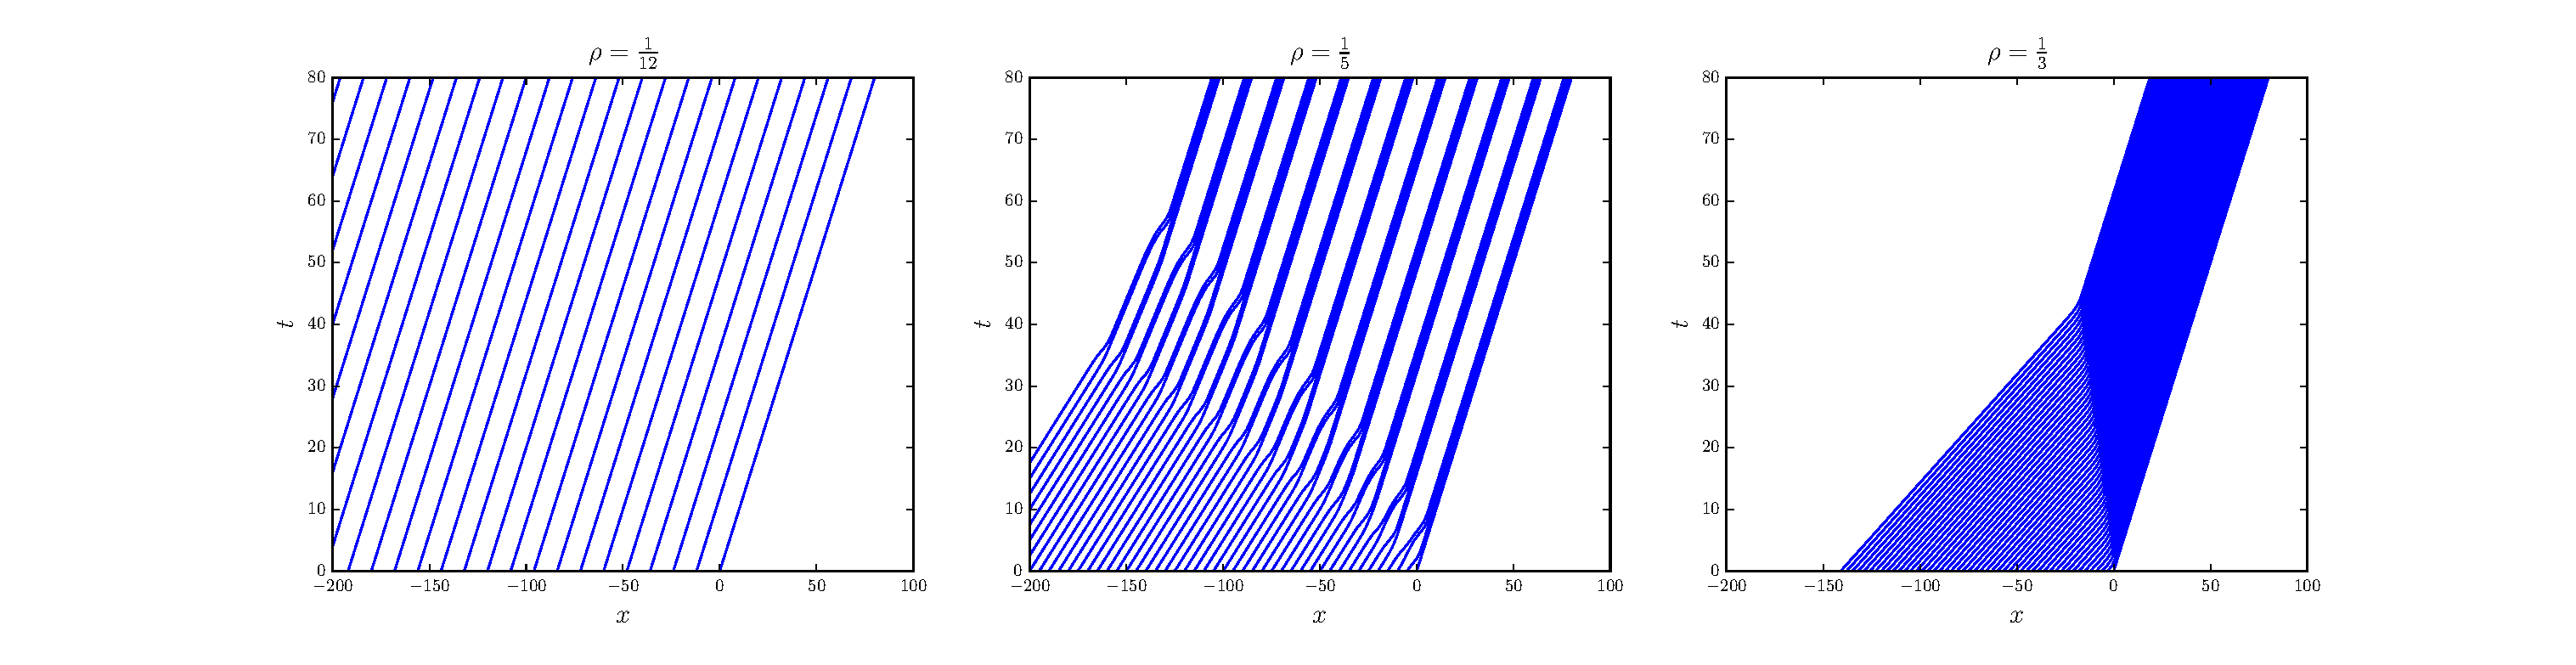
\includegraphics[width=7in]{./figs/night_cluster.eps}
%----------------------------------------------------------
\subsection{Random Perturbation}

However, on the real road, it is not realistic that cars group into platoons of same number. In order to simulate this phenomenon, random perturbation can be added to adjust the velocity,
\[v_{n+1}(t)=U(\rho_{n+1}(t))+A\epsilon,\]
where $\epsilon$ is a random variable with uniform distribution on $[-0.5,0.5]$, and $A(t)$ is the amplitude of the perturbation. Since crash of cars are not expected, the amplitude $A(t)$ needs to be constrained.

Assume $x_1$ is the leading car. To update the positions,
\begin{align*}
&\left\{\begin{array}{lll}
x_{n+1}(t+\Delta t)=x_{n+1}(t)+\Delta t(U(\rho_{n+1}(t))+A(t)\epsilon_1)\\
x_{n}(t+\Delta t)=x_{n}(t)+\Delta t(U(\rho_{n}(t))+A(t)\epsilon_2).
\end{array}\right.
\end{align*}

In the following part, we will denote $U_n(t)=U(\rho_n(t))$. By taking the difference between the equations above, we have
\[
x_n(t)-x_{n+1}(t)+\Delta t (U_{n}(t)-U_{n+1}(t))+A(t)(\epsilon_1-\epsilon_2)>0.
\]

Let $\epsilon_1=0.5$ and $\epsilon_2=-0.5$,
\[A(t)<\frac{x_{n}(t)-x_{n+1}(t)}{\Delta t}+[U(\rho_{n}(t))-U(\rho_{n+1}(t))].\]

This is our restriction on amplitude.
\vskip 1cm
%----------------------------------------------------------
{\bf Car-Following Simulation}
\\

We use the same parameters as above.

\hspace*{-1in}
\hfil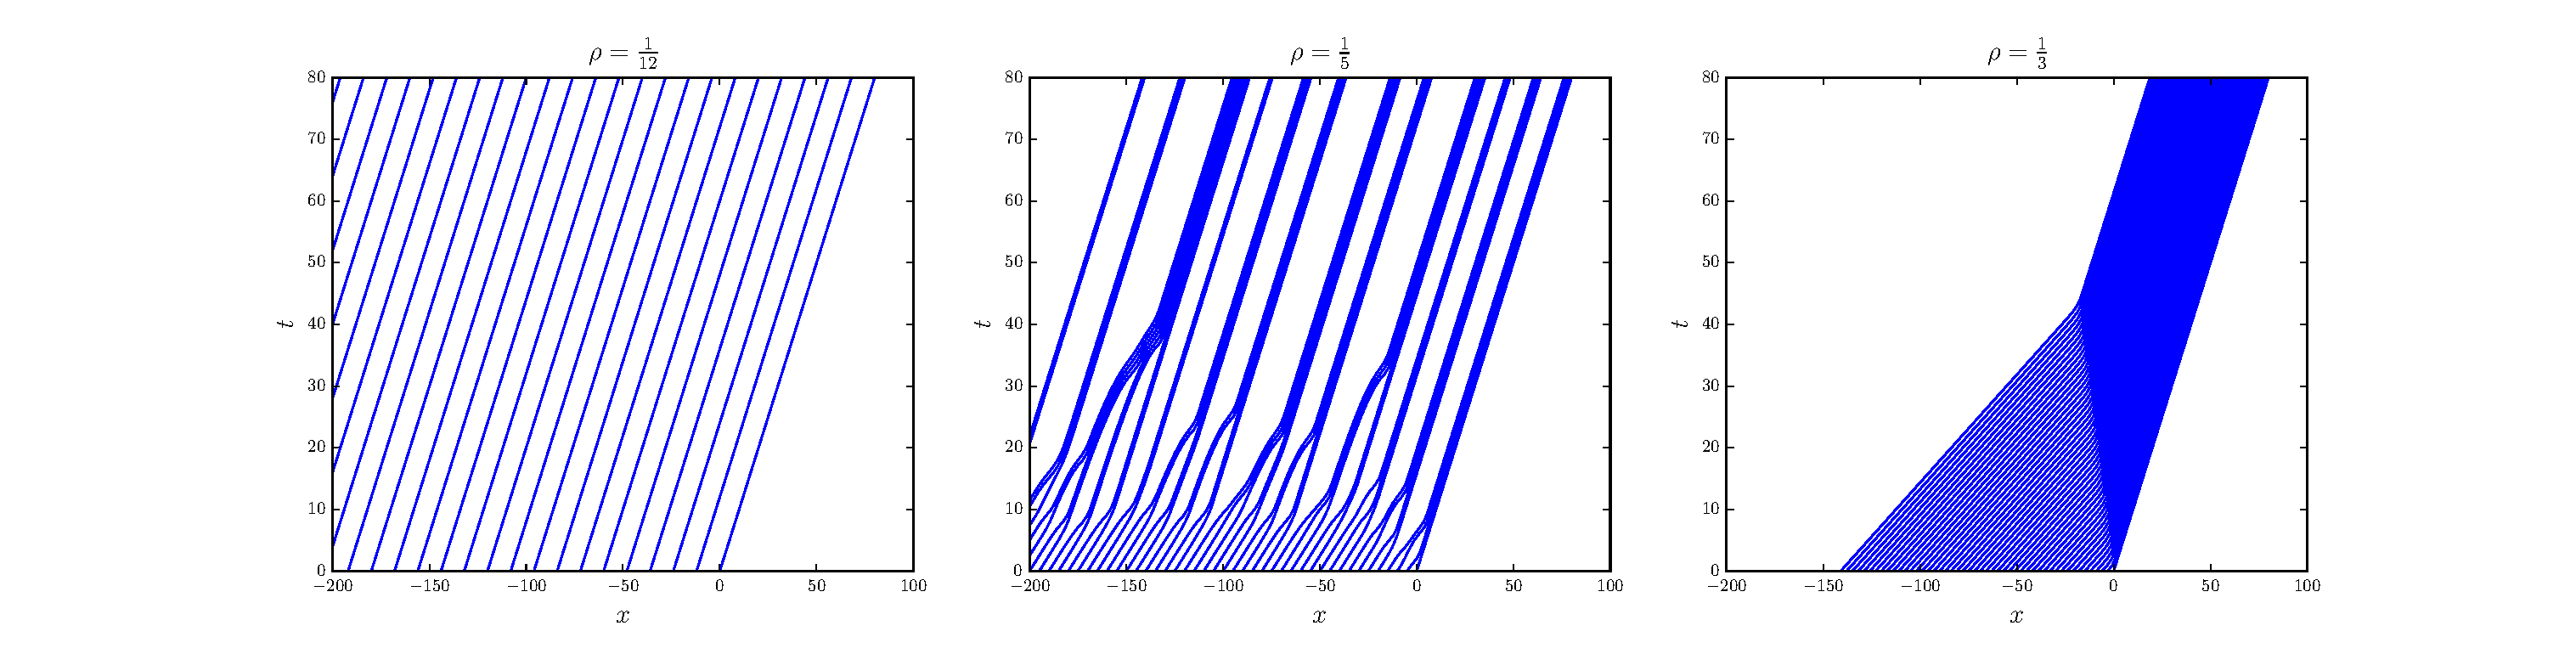
\includegraphics[width=7in]{./figs/night_cluster_rand.eps}
%----------------------------------------------------------
\subsection{Discussion}
Without perturbation, cars are easily grouped into pairs, which is called platoon solution in \cite{RJ}, where LeVeque explains, ``The lead driver sees $\rho=0$ and drives at speed $v_0$, and then the second driver initially sees $\rho=\rho_0$ and can drive faster. But as the second car accelerates, the third driver observes a drop in density and hence this driver starts to slow down. This causes the fourth driver to go faster.''

\vskip 8pt
With random perturbations, we can observe platoons with different number of cars, which is much more reasonable to simulate
the real night-time driving behavior.
%-----------------------------------------------------------------------------------------------------------------------%
\section{Conclusion}

In this paper, we talk about two different models of traffic flow. Based on Olenik's entropy condition, which is originally for the fluid problem, the convex hull is constructed to solve freeway model. In \cite{Z}, Zhang set two mathematical criteria for anisotropic model, and Wiens proved that this freeway model satisfies these requirements in \cite{WJ}. From the results of car-following model, we can see that even if this model is anisotropic (while fluid is isotropic), convex hull method still gives a good result. However, it is not true for night-time driving model \cite{RJ}. In the second part, we investigate the night driving behavior with random perturbations, which gives reasonable results in reality. In the future, we would like to look into new entropy condition and numerical solutions for this problem.

%-----------------------------------------------------------------------------------------------------------------------%
% references
{\footnotesize
\begin{thebibliography}{100}
\bibitem{RJ} LeVeque, R. J. (2001). Some traffic flow models illustrating interesting hyperbolic behavior. Minisymposium on traffic flow.
Chicago.
\bibitem{WS} Wiens, J. K., Stockie, J. M., \& Williams, J. F. (2013). Riemann solver for a kinematic wave traffic model with discontinuous flux. Journal of Computational Physics, 242, 1-23.
\bibitem{JW} Jiang, R., \& Wu, Q. S. (2007). The night driving behavior in a car-following model. Physica A: Statistical Mechanics and its Applications, 375(1), 297-306.
\bibitem{DF} Dias, J. P., \& Figueira, M. (2005). On the approximation of the solutions of the Riemann problem for a discontinuous conservation law. Bulletin of the Brazilian Mathematical Society, 36(1), 115-125.
\bibitem{Z} Zhang, H. M. (2003). Anisotropic property revisited��does it hold in multi-lane traffic. Transportation Research Part B: Methodological, 37(6), 561-577.
\bibitem{WJ} Wiens, J. K. (2011). Kinematic wave and cellular automaton models for traffic flow (Doctoral dissertation, Science: Department of Mathematics).
\end{thebibliography}
}
\end{document}
\end{document}

